Use case 1, figur \ref{fig:UC1} og tabell \ref{tab:UC1}, beskriver arbeidsflyten til en 
lastebilsjåfør for å oppdage et varsel om et løst hjul på en 
smartskjerm innstallert i dashbordet i lastebilen.
\newline
\begin{figure}[H]
	\centering
	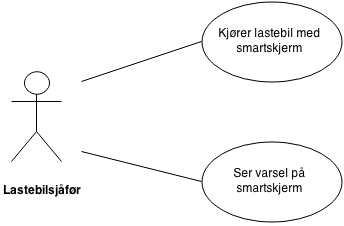
\includegraphics[width=0.50\textwidth]{images/UC1.png}
	\caption{Use case 1: Sjåfør oppager varsel.}
	\label{fig:UC1}
\end{figure}

\begin{table}[H]
\caption{Use case 1}
\label{tab:UC1}
\begin{tabularx}\linewidth{ |m{0.3 \textwidth} |X|   }
	\hline
	ID	& 1 \\
	\hline
	Navn	& Oppdage varsel \\
	\hline
	Mål	& Oppdage varsel om løs mutter på smartskjerm\\
	\hline
	Aktører	& Lastebilsjåfør\\
	\hline
	Precondition	& Ingen \\
	\hline
	Prerequisite	& En smartskjerm er innstallert i dashbord i lastebilen\\
	\hline
	Hovedflyt 	&  1. Kjører langs veien \\
				&  2. Gløtter bort på smartskjermen \\
				&  3. Oppdager varsel \\
	\hline
	Alternativ Flyt	& Ingen\\
	\hline
	Foregående UC	& Ingen\\
	\hline
	Følgende UC	& UC2\\
	\hline
\end{tabularx}
\end{table}
%
Use case 2, figur \ref{fig:UC2} og tabell \ref{tab:UC2}, beskriver dataflyten fra hjulenhet, gjennom 
prosesseringsenheten, og til smartskjerm innstallert i dashbordet i 
førerhuset i en lastebil. 
\newline
\begin{figure}[H]
	\centering
	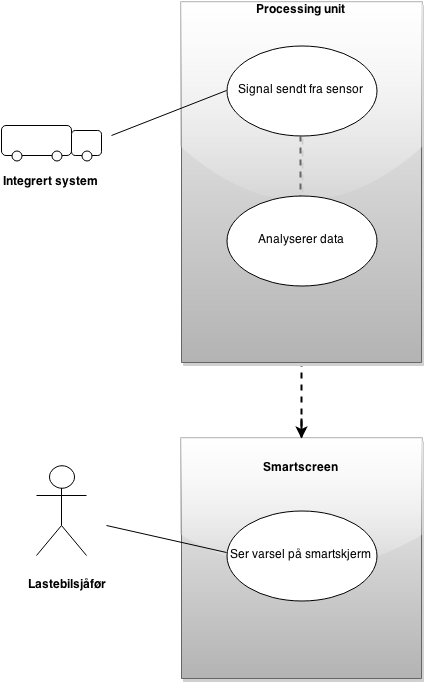
\includegraphics[width=0.50\textwidth]{images/UC2.png}
	\caption{Use case 2: Signaler prosesseres og sendes til førerhus.}
	\label{fig:UC2}
\end{figure}

\begin{table}[H]
\caption{Use case 2}
\label{tab:UC2}
\begin{tabularx}\linewidth{ |m{0.3 \textwidth} |X|   }
	\hline
	ID	& 2 \\
	\hline
	Navn	& Signaler sendes \\
	\hline
	Mål	& Prosessere signaler sendt fra hjulenhet til førerhus\\
	\hline
	Aktører	& Integrert system, lastebilsjåfør\\
	\hline
	Precondition	& Ingen \\
	\hline
	Prerequisite	& Sentralt system innstallert i lastebil\\
	\hline
	Hovedflyt 	&  1. Signal sendes fra hjulenhet til prosesseringsenhet \\
				&  2. Signal prosesseres \\
				&  3. Formatert signal sendes til smartskjerm \\
				&  4. Sjåfør oppdager feilmelding \\
	\hline
	Alternativ Flyt	& Ingen\\
	\hline
	Foregående UC	& UC1\\
	\hline
	Følgende UC	& Ingen\\
	\hline
\end{tabularx}
\end{table}